\documentclass{article}
\author{Wenzhao Xu, Haoyan Cai}
\title{STAT 542 Final Project Proposal}
\usepackage{amsmath}
\usepackage{graphicx}
\usepackage{subfig}
\usepackage{multirow}
\usepackage[top=1in, bottom=1in, left=1.25in, right=1.25in]{geometry}

\begin{document}
	\maketitle
	
	\section{Introduction} % (fold)
	\label{sec:introduction}
	
	\paragraph{} The data are about accelerometer data from mobile devices. The train data contain X,Y,Z direction acceleration values from 387 devices and testing data set have 90024 testing sequences. For each test sequence, we have information of a possible device. The goal is to judge whether this possible device is the true device that generate the test sequence. 
	% section introduction (end)
	
	\section{Data Set} % (fold)
	\label{sec:section_name}
	\paragraph{}
	Package "ff" and SQL database can be used to import data from a large csv file. Unix time is then converted to standard GMT time. A typical visulization of data is shown in Figure 1, in which Device 7 is a device with long sampling time and total 523187 points while Device 770 has limited sampling points as 28475.
	\begin{figure}
		\centering
		\subfloat[Device 770]{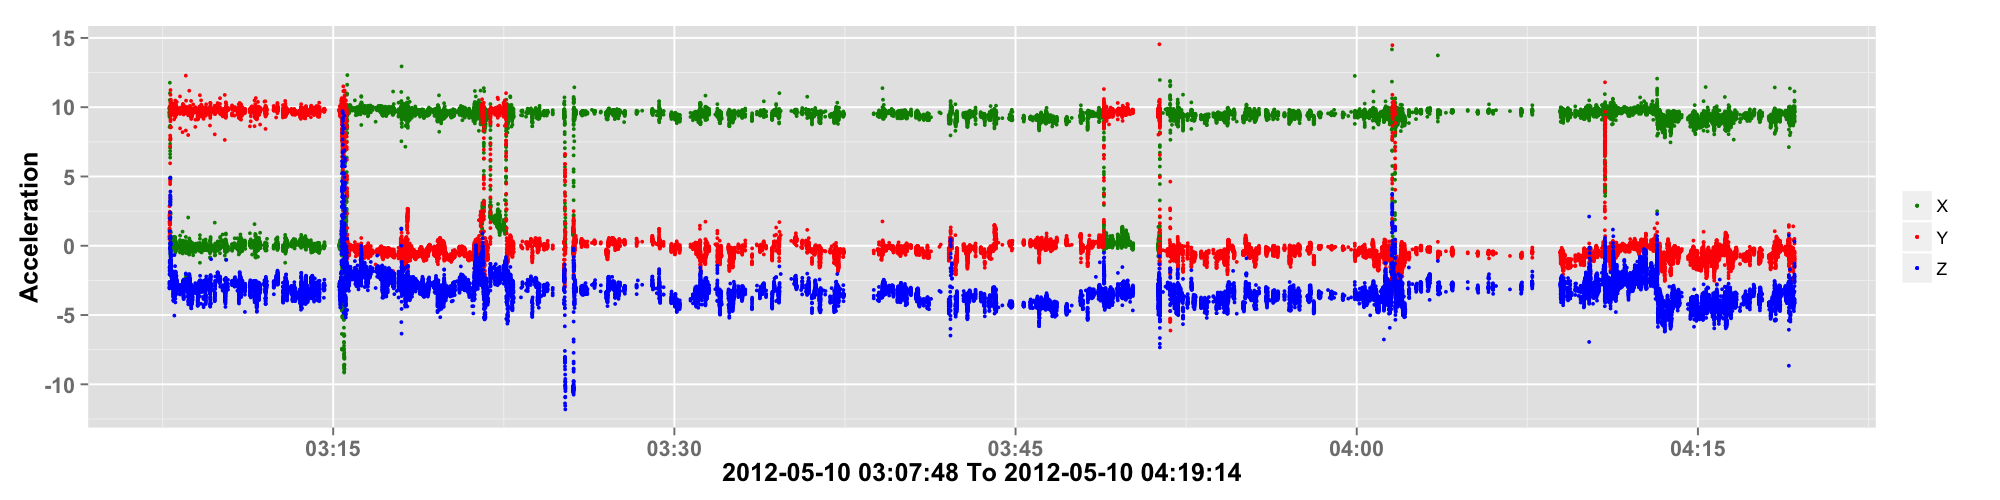
\includegraphics[width=1\textwidth]{photoshare/770.png}}\\
		\subfloat[Device 7]{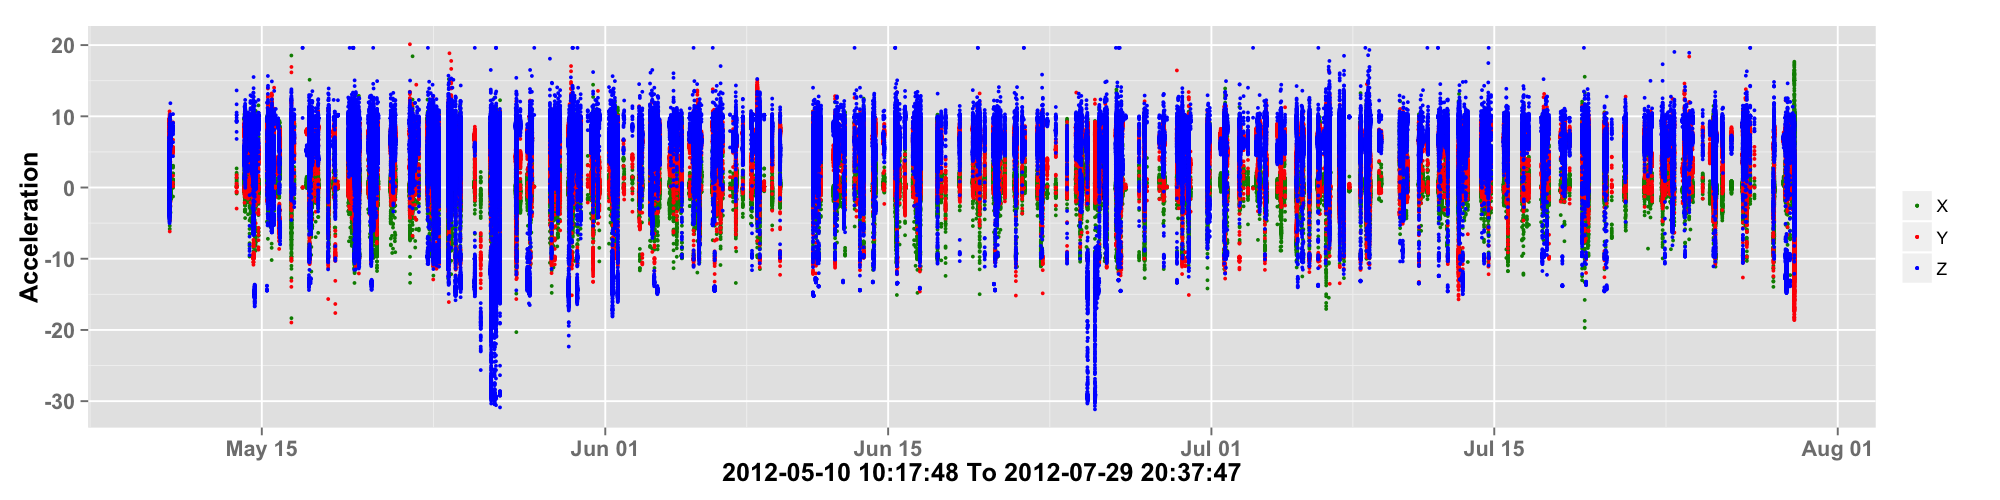
\includegraphics[width=1\textwidth]{photoshare/7.png}} \\
		\caption{Acceleration Data Along Time}
	\end{figure}
	
	\paragraph{}In test data, each sequence contains 300 sampling points, roughly lasts for less than 1 minute. We need to identify whether the professed device in the test sequence is the true device. Figure 2 shows two sequence whose professed device are 770. Compared with the train data from device 770 (Fig 1(a)), it seems sequence 838966 is likely belong to device 770 while sequence 690194 is not since the range of X,Y,Z in sequence 838966 is consistent with training data from device 770. 
	\begin{figure}
		\centering
		\subfloat[Sequence 690194]{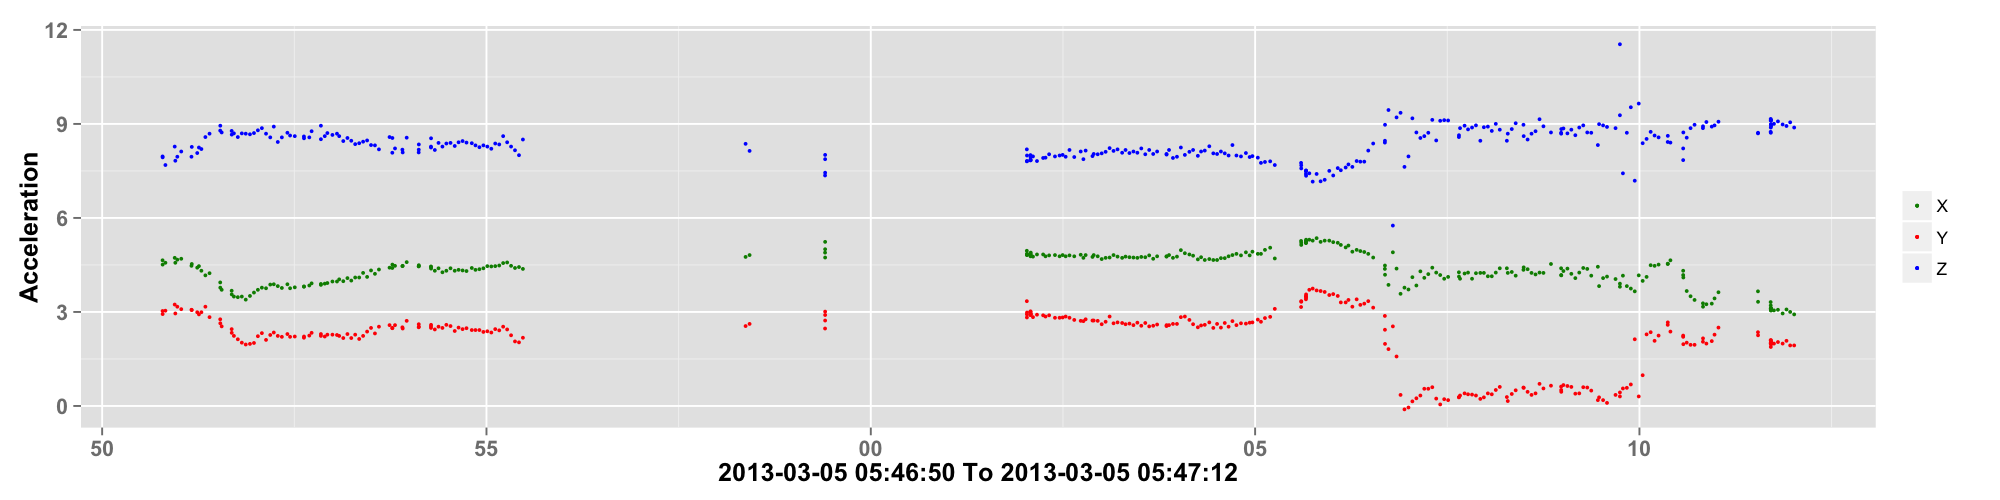
\includegraphics[width=1\textwidth]{photoshare/690194.png}}\\
		\subfloat[Sequence 838966]{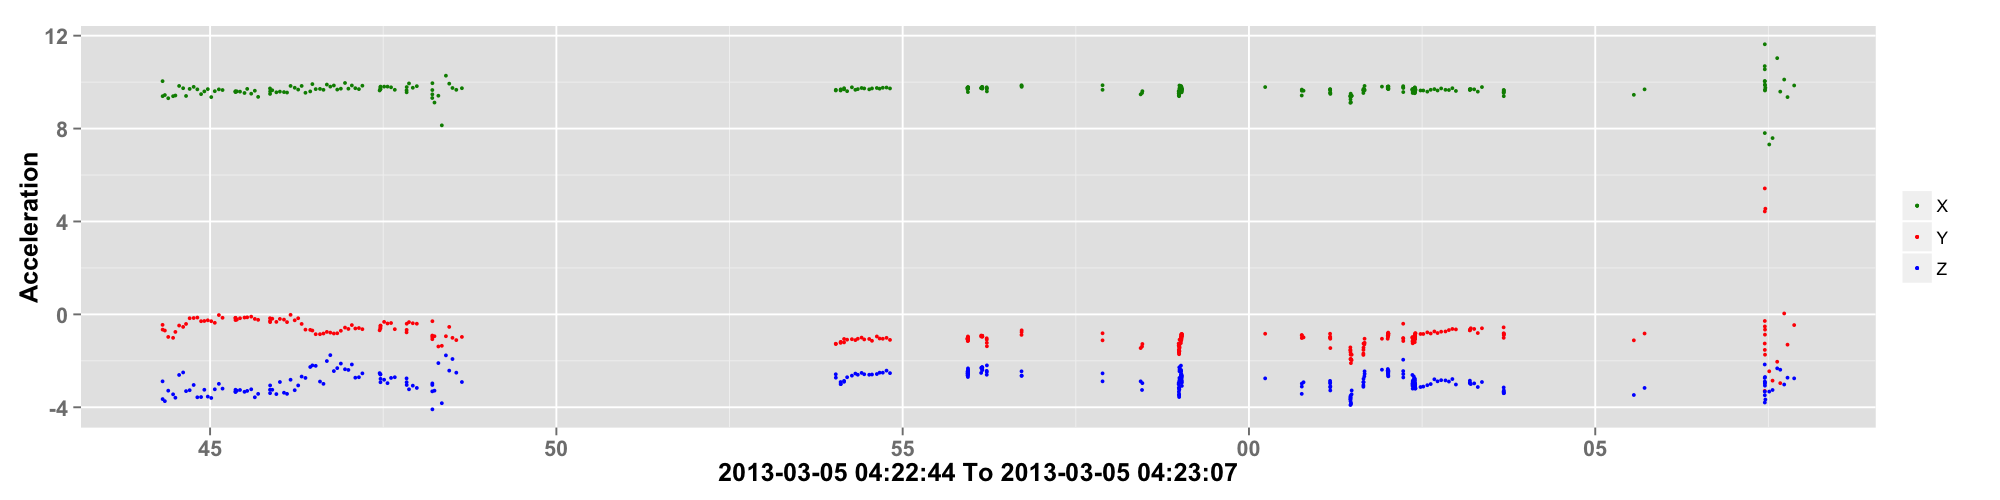
\includegraphics[width=1\textwidth]{photoshare/838966.png}}
		\caption{Test Sequence with Professed Device as 770}
	\end{figure}
	
	% section section_name (end)
	

	\section{Potential Approach} % (fold)
	\label{sec:potential_approach}
	\paragraph{}The data involve with time dimension, which is a very important feature. To solve this problem, an assumption should be made that users' activities have similarity. Similarity means users are likely to have similar behavoir during similar time of day. For example, users would have similary X,Y and Z time series during today's 4:00pm and yesterday's 4:00pm. 
	\paragraph{} Based on this assumption, we design the following approach:
	\begin{itemize}
		\item First, approtiate features from the raw data should be defined. Some simple but probably useful features include the range of X,Y,Z, the difference between X and Y, between X and Z, and between Y and Z, autocorrelation of X,Y and Z, and correlations between X,Y and Z, etc. In addition, We plan to do some literature research about what activities the data might reveal in order to extact features that represent users personal habbit such as how he/she runs. 
		\item Second, one big problem is that how we define the probability for a test sequence to be rejected. Since data are generated by different time, training data might have different patterns during different time period. So given a test sequence $X_{test}$, we denote its time of day as $T_{test}$ (e.g. $T_{test}=19:00$). Then search all the training data and extract available training sequences (denote as $X_{train}$) that were generated close to $T_{test}$. For the test sequence $X_{test}$, a professed device $D$ is known. We can label the training sequences from device $D$ as 1 and the training sequence from other device as 0. Based on the features we extract, train some classifier models with these training sequences and get the classifiers. Finally, apply the classifier to the test sequence to see wether it is 0 (test sequence is belong to other device) or 1 (test sequence is belong to device $D$). It should be noticed that identifying what activity the test sequence represents such as running or walking or sleeping is also important. If the test sequence is from running but the running pattern from professed device is total different with what test sequence reveals, then the professed device is probably a wrong device. 
		
	\end{itemize}
	
	\section{Timeline} % (fold)
	\label{sec:timeline}
	\begin{itemize}
		\item Research on literatures with acceleration data
		\item Extract important features 
		\item Initial result done (before the end of thanksgiving holiday)
		\item Improve result
	\end{itemize}
	% section timeline (end)
	
	% section potential_approach (end)
	
\end{document}




